\par{\emph{Host} connected to one or more OpenCL \emph{devices}. One or more 
    \emph{compute units} belong to one OpenCL \emph{device}, and one \emph{compute unit} is divided into one or more
    \emph{processing elements}. The \emph{processing elements} in a \emph{compute unit} execute a single stream of instructions
    as SIMD units(execute in lockstep with a single stream of instructions) or SPMD units(each \emph{processing element} 
    maintains its own program counter), this model is shown in figure \ref{PlatformModel}\cite{opencl12}.}

\begin{figure}[!h]
    \centering
    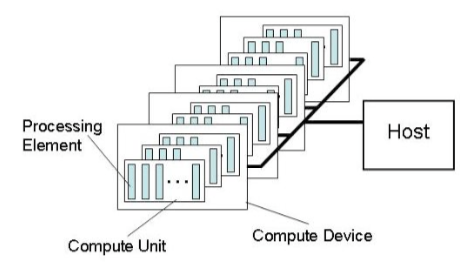
\includegraphics[width=0.4\textwidth]{figures/PlatformModel.png}
    \caption{Platform Model\cite{opencl12}.}
    \label{PlatformModel}
\end{figure}

